\documentclass{bmvc2k}

%% Enter your paper number here for the review copy
\bmvcreviewcopy{134}

\title{skeleton based action recognition\\ using few shot learning}
\usepackage{amsfonts}
\usepackage[ruled]{algorithm2e}
% Enter the paper's authors in order
% \addauthor{Name}{email/homepage}{INSTITUTION_CODE}
%\addauthor{Susan Student}{http://www.vision.inst.ac.uk/~ss}{1}
%\addauthor{Petra Prof}{http://www.vision.inst.ac.uk/~pp}{1}
%\addauthor{Colin Collaborator}{colin@collaborators.com}{2}

% Enter the institutions
% \addinstitution{Name\\Address}
\addinstitution{
% The Vision Institute\\
% University of Borsetshire\\
% Wimbleham, UK
}
\addinstitution{
% Collaborators, Inc.\\
% 123 Park Avenue,\\
% New York, USA
}

\runninghead{Student, Prof, Collaborator}{skeleton based action recognition using few shot learning}

% Any macro definitions you would like to include
% These are not defined in the style file, because they don't begin
% with \bmva, so they might conflict with the user's own macros.
% The \bmvaOneDot macro adds a full stop unless there is one in the
% text already.
\def\eg{\emph{e.g}\bmvaOneDot}
\def\Eg{\emph{E.g}\bmvaOneDot}
\def\etal{\emph{et al}\bmvaOneDot}

%-------------------------------------------------------------------------
% Document starts here
\begin{document}

\maketitle

\begin{abstract}
This paper presents a new skeleton-based action recognition method using a few shot learning. Consider the sequence data contain the temporal and spatial information; the proposed method encodes each of skeleton as an RGB image. Nothing more but a naïve normalization is engaged to each channel of the encoded skeleton image. In order to acquire the discriminative feature of skeleton image, dilated-dense layer is adopted in our model to both extend the receptive field of feature points and capture diversity representation of the skeleton image. After that, the prototypical network is introduced to recognize the specific action of the feature stands for. It can map the skeleton image into a metric space in which action classification can be performed by the nearest neighbor search. Benefited from the nature of the few shot learning, our model can be trained with only a few training samples. Moreover, it can adjust to the new classes that had not presented during the training phase with a few labeled samples from unseen classes. We evaluated our method with the seen and unseen class of samples, experiment result shows, the method achieved comparable performance on benchmark datasets.

\textbf{Index Terms:} skeleton sequence, dilated-dense layer, few shot learning
\end{abstract}

%-------------------------------------------------------------------------
\section{Introduction}
\label{sec:intro}
Human action recognition has been widely researched for a few decades. A lot of action recognition methods are developed to serve for entertainment, surveillance, and video analysis. Recently, the methods has made a great step forward by the wave of the deep learning. However, these deep learning based methods usually consume large-scale of training samples to capture the inner pattern of every action. As human action category is varied, the demand for training samples will explode. Besides, when new unseen actions are acceded to the classification task, the deep model need to be retrained for changing quantity of the action. A kind of few-shot (one-shot, zero-shot) learning methods are proposed to resolve these issues. Usually, these method can quickly accommodate the new classes by given a few of labeled samples from new class. Instance-based learning, Non-parametric method, meta-learning and metric learning~\cite{davis2007information} have played a significant role in the progress of this field. Mishra~\cite{mishra2018generative} present a generative framework for Zero-Shot or Few-Shot action recognition. Yang~\cite{yang2018one} introduce a new example-based action detection based on the Matching Network. Nevertheless, seldom attention had been paid to apply the few shot learning model to skeleton sequence yet. To address this challenge, we propose an action recognition method based on the prototypical network. It can learns a metric space in which classification can be performed by computing distances to prototype representations of each class ~\cite{snell2017prototypical}. The performance of our method also benefits from convolution network, because we had engaged a serial of convolution layers to extract the feature of skeleton sequence. And The main contributions of this method are:

\textbf{1.}Only a few skeleton sequence samples are adequate to train an efficient action recognition model.

\textbf{2.}With a few support samples, the model is capable of recognizing the new action that had not seen during the training period.

\textbf{3.}	Dilated-dense layer is embedded to our model, which can enhance the robustness and diversity of the skeleton feature representation. 

The remainder of the paper is organized as follows. In Sec.2 we briefly review methods proposed to deal with skeleton-based action recognition. In Sec.3 a simple encoder without bells and whistle is introduced to encode the sequence as a skeleton image. Then a convolution network with dilated-dense layers is designed to map the skeleton image into a suitable metric space. Finally, we fully describe the training and recognition process of our action recognition method. In Sec.4 we report the experiments results on two datasets to show the performance of the method with a few-shot samples. In Sec.5 we discuss research directions in the future work.

\begin{figure}[htb] 
	\centering
	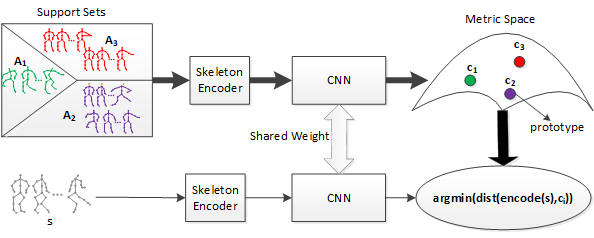
\includegraphics[height=1.8in]{images/Figure_1.png}
	\caption{Proposed Model: The support sets (a few labeled sequences) are mapped into a metric space to estimate the prototype of each class. During the training phase, the convolution network with dilated-dense layers is learned as the mapping function. And for the inference, the unlabeled sample $s$ is assigned to the class whose prototype has the shortest distance from it in the metric space.}
	\label{fig:1}	
\end{figure}
\section{Related Work}

Skeleton sequence data contains strong interpretive feature for the action recognition task. A rich of deep action recognition models had proposed on such kind of data. Specifically, these methods can be sumaried as three main streams. 
The first streams usually encode the skeleton sequence into a skeleton-image. Different skeleton-image encoders are proposed to capture the feature of actions. Wang~\cite{wang2016action} introduce a compact and effective method to encode spatiotemporal information carried in 3D skeleton sequences into a Joint Trajectory Maps (JTM). Pham~\cite{pham2017learning} and Li~\cite{li2017skeleton} rearrange the pixels in RGB skeleton images to obtain a better representation of the movement. Furthermore, Liu~\cite{liu2017enhanced} design a skeleton visualization method to represent a skeleton sequence as a series of visual and motion enhanced color images. Having encoded skeleton sequences into skeleton images, a variety of CNN networks(CNN~\cite{wang2016action}, multi-scale CNN~\cite{li2017skeleton_2}, DeepResidualNeuralNetworks~\cite{pham2017learning}, multi-stream CNN~\cite{liu2017enhanced}) are constructed to classify the indeed action of the skeleton image. 

The second steam is inspired by the RNN network, whose recurrent structure can boil a sequence data down into a high-level understanding ~\cite{olah2016attention}. For better performance, they tend to adopt the LSTM to process the skeleton sequence data. Zhu~\cite{zhu2016co} introduce an end-to-end fully connected deep LSTM network with a designed regularization, through which can learn the co-occurrence feature of the skeleton joints. Based on LSTM, Liu~\cite{liu2018skeleton} design a skeleton tree traversal method and a new gating mechanism to achieve a robust representation of the input sequence data. To further, Liu~\cite{liu2018skeleton_13} also add attention ability to the LSTM network, which is capable of focusing on the informative joints of the skeleton.
The last one is based on graph convolutional network ~\cite{bruna2013spectral}, which can be applied directly to the raw skeleton data. Shi\cite{shi2018non-local} present a novel two-stream nonlocal graph convolutional network for the recognition task. Li~\cite{li2018spatio} proposed a spatio-temporal graph convolution approach with multi-scale kernels to recognize the actions. Si\cite{si2019attention} proposes a novel Attention Enhanced Graph Convolutional LSTM Network, which can not only capture discriminative features in spatial configuration and temporal dynamics but also explore the co-occurrence relationship between spatial and temporal domains.
\section{Proposed Method}
\subsection*{Skeleton Image Encoder}
It is common knowledge that a skeleton sequence can be represented as an RGB image. Consider an $n$ frame skeleton sequence $s=\{ fr^1,fr^2,\cdots fr^n\}$, each frame $fr^i$ includes $m$ joints $fr^i =\{j^i_1,j^1_2,\cdots j^i_m\}$ And each joint $j^i_t=\{j^i_{tx},j^i_{ty},j^i_{tz}\}$  is a 3-D coordinate point, which is corresponding to the RGB channel of a pixel in a skeleton image. Thus, the skeleton sequence S can be encoded as an $m\times n$ skeleton image. a sort of variant RGB encoder had proposed to achieve the translation-scale invariant representation of the skeleton sequences~\cite{liu2017enhanced,ke2017new}. But our model hasn’t taken advantage of these mechanisms. Only a naive normalization, proposed by ~\cite{chen2015utd}, is adopted.

$$p'_k=floor(255*\frac{(p_k-p^{min}_k)}{\max \limits_{k}(p_k^{max}-p_k^{min})})$$

Where $p^{max}_k$ and $p^{min}_k$ are the maximum and minimum value of the k-th channel $(x; y; z)$ of a skeleton. In this way, each skeleton $s$ can be encoded into a skeleton image $I$. 

\begin{figure}[htb] 
	\centering
	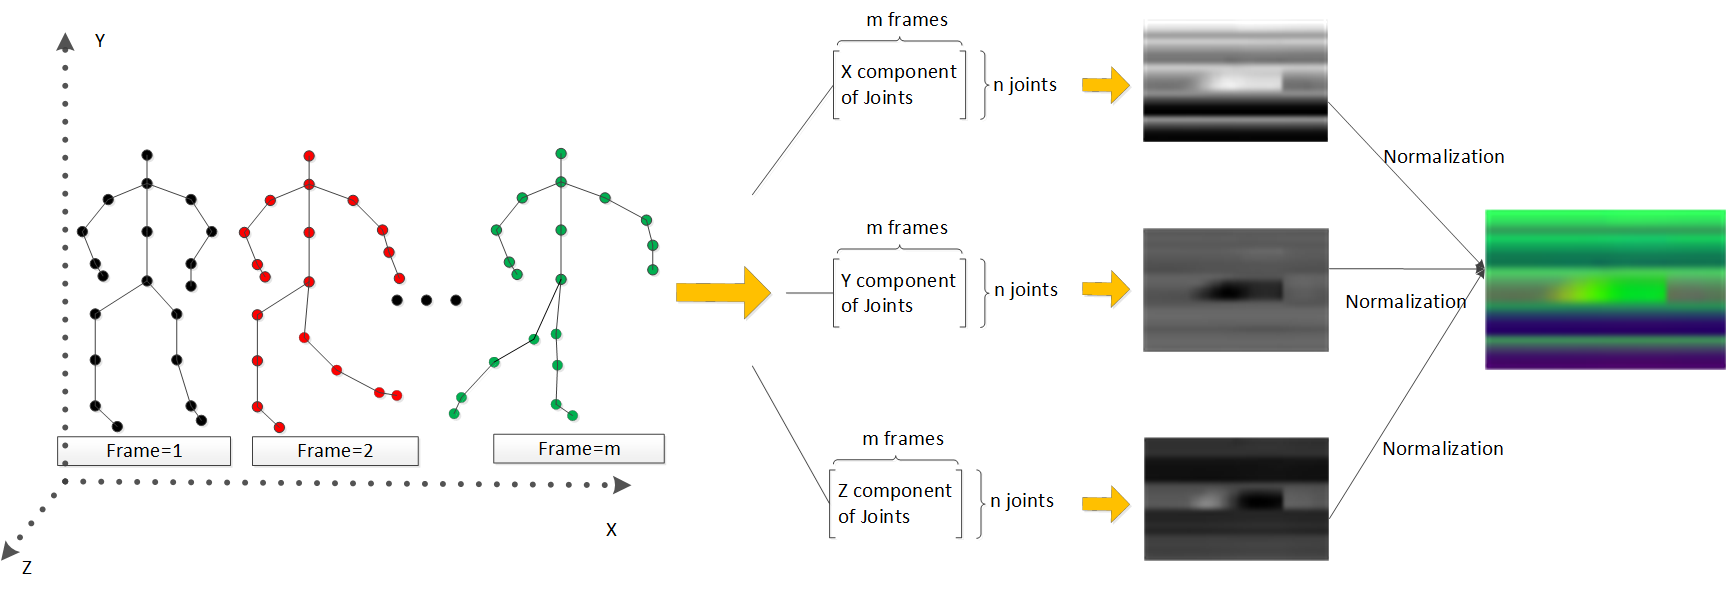
\includegraphics[scale=0.25]{images/Figure_2.png}
	\caption{The workflow of the encoder. each component of the skeleton joints in a sequence is encoded as a channel of the RGB image. And the normalization is applied independently to each channel to generate the final skeleton image.}
	\label{fig:2}	
\end{figure}

\subsection*{The Mapping Function}
Having the skeleton sequence encoded as an RGB image, we will map it into a metric space via a mapping function $F_W:\mathbb{R}^D\rightarrow \mathbb{R}^M$. The function is the learnable part of our action recognition model. For the sake of processing the RGB skeleton image, we construct the mapping function as a convolution network. There are two things that we considered before build the network. One is that, unlike natural image, each pixel scattered in the image has equally interpretive meaning for the final decision, we tend to expand the size of the convolution kernel, so that is can convolve as much as pixels in the skeleton image. The other one is that, both the movement of the skeleton joints in temporal domain and the configuration of the joints in spatial space are the powerful features of action. For these reasons, we considered adding dilated-dense layers, whose dilated convolution kernel could enlarge the receptive field of the feature point and the densely connected layers can lead to a rich of configuration and movement feature representation. 

\begin{figure}[htb] 
	\centering
	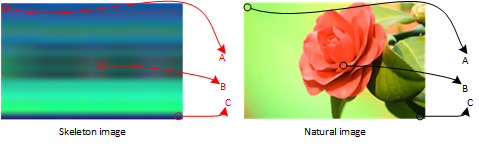
\includegraphics[scale=0.8]{images/Figure_3.png}
	\caption{Each pixel represents a skeleton joint in skeleton image. Even the pixel around the corner(A,C) has equally importance to the one(B) located in the center. While things usually do not happen in natural image.}
	\label{fig:3}	
\end{figure}

\begin{figure}[htb] 
	\centering
	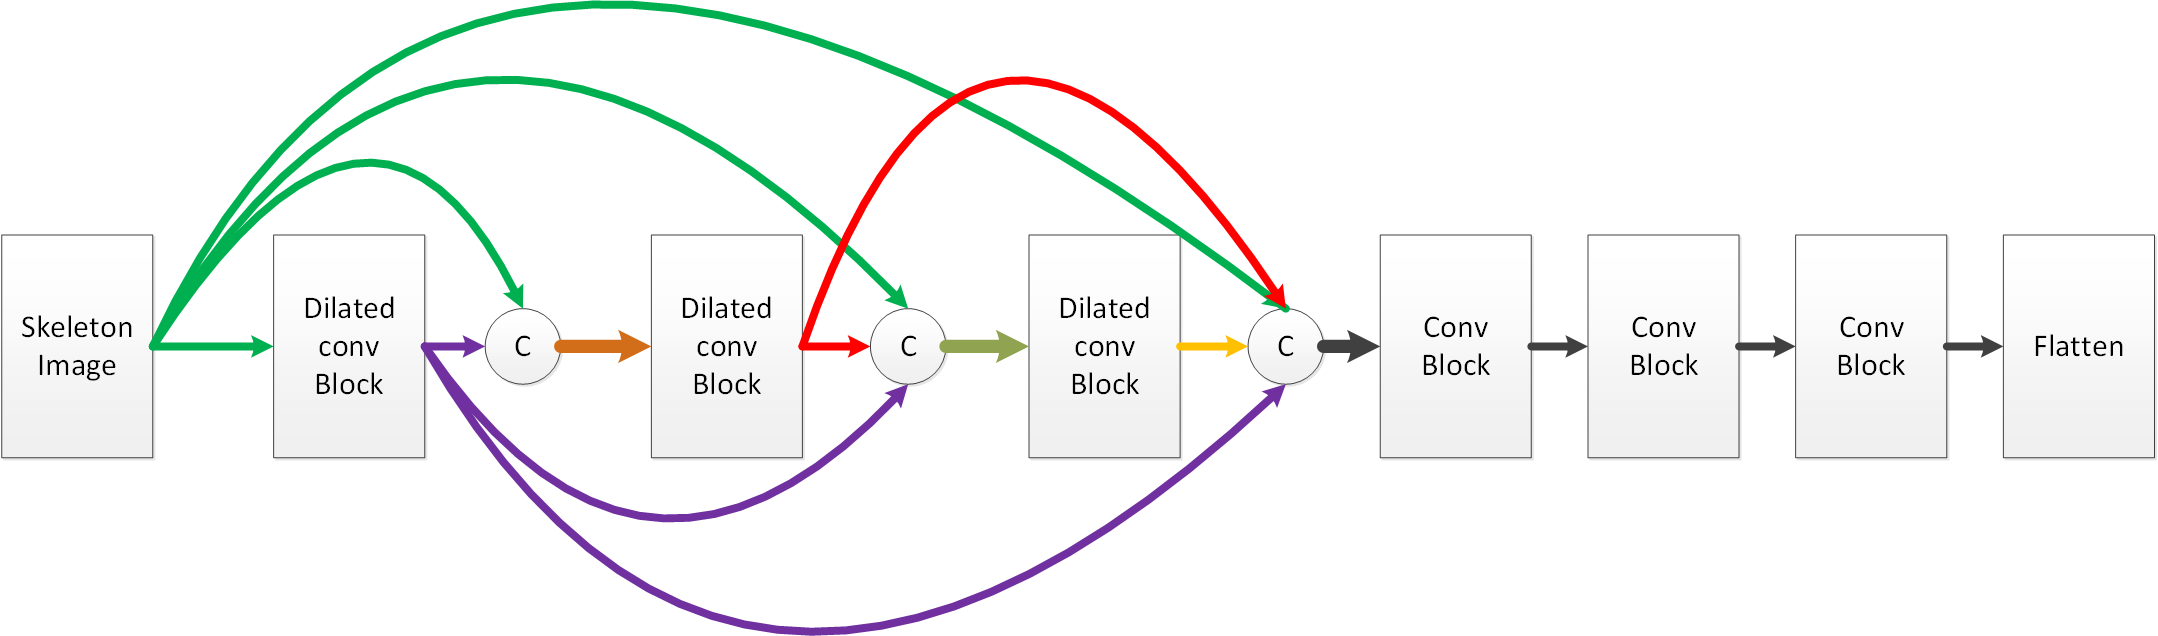
\includegraphics[scale=0.2]{images/Figure_4.png}
	\caption{The architecture of the mapping function $F_W$. The first three dilated-conv-dense blocks are designed to enhance the robust representation of the skeleton image. Meanwhile, the later three convolution blocks are for projecting the feature into a discriminative space. And the final flatten layer will convert the feature into a one-dimension tensor. Weights and biases of the network are corresponding to the parameter of the mapping function.}
	\label{fig:4}	
\end{figure}

\subsection*{The Model}
Figure \ref{fig:1} illustrate the whole structure of the action recognition model. our model includes two independent parts of parameters. One is the prototype of the classes $C_{support}=\{c_1,c_2,\cdots c_K\}$. it can be estimated by calculating the mean of the support set samples in metric space. The other one is the parameter of the mapping function $F_W$, which can be solved via SGD optimization. Given $K$ classes of labeled skeleton samples, we randomly subsample a few of data from each class as the support sets. The k-th support set can be defined as:

$$S_k=s_1,s_2,\cdots s_{N_s}$$

The support sets will be mapped into a metric space by the convolution layers and the prototype of k-th class $c_k$ is the mean of the mapped support samples that belong to it. 

$$c_k=\frac{1}{N_s} \sum \limits_{s_i,y_i\in S_k}F_W (encode(s_i))$$

When feeding an unlabeled skeleton image $s^*$, the label of the image is decided by the nearest neighbour prototype, from whom it has the shortest distance.

$$\mathop{\mathbf{argmin}}_{i} ( \lVert F_W ( encode(s^\ast) ) - c_i \rVert^2 )$$

The inference phase of our model is similar to the nearest neighbor search. Algorithm \ref{alg:1} is a brief pseudo-code of the inference phase.


\begin{algorithm}
	\caption{ the inference process of action recognition model.}
	\KwIn{$k$ classes of support set $S=\{S^1,S^2,\cdots S^k \}$, where each class of support}
	\KwOut{the assignment of the unlabeled sample $y^*$}
	\label{alg:1}
	\ForEach{\bf{i in K}}
	{
		
		$\mathbf{I^i}=\{I^i_1,I^i_2,\cdots I^i_N\}=\mathbf{encode}(S^i)$
		
		$\mathbf{F^i}=\{F^i_1,F^i_2,\cdots F^i \{ N_s \} \}=\mathbf{F_w(I^i)}$
		
		$\mathbf{c_i}\leftarrow \mathbf{mean}(F^i)$
		
	}
	
	$I^\ast = \mathbf{encode}(a^\ast) $
	
	$F^\ast = \mathbf{F_w}(I^\ast)$
	
	$y^\ast=\mathop{\mathbf{argmin}}\limits_{\mathbf{i}} \left( \lVert F_W \left( I^\ast \right) - c_i \rVert^2 \right)$
\end{algorithm}

The purpose of our training algorithm is to address the learnable parameter of $w$. To training the model, the labeled samples are divided into support and query sets. Support sets are used to estimate the prototype of each classes. While the query sets are used to calculate the loss of the model. For each labeled query sample $(s^\ast,y^\ast)$, The cross-entropy loss of the prototypical model can be defined as:

$$loss(y=y^\ast | s^\ast,C_{support},W)=\log(\frac{\exp (-d(F_W(encode(s^\ast)),c_{y^\ast}))}{\sum_{i=1}^{k}\exp((F_W(encode(s^\ast)),c_i)})$$

Figure \ref{fig:4} illustrates the detail computation of the cross-entropy loss of the model. Having the loss function defined, we optimize the parameters of the model in few shot fashion. For each training iteration, we randomly divided the labeled samples into the support and query set. With which the cross-entropy loss of the model will be calculated to updated the parameter of the network. A detail description of training phase is provided in algorithm \ref{alg:2}.

\begin{figure}[htb] 
	\centering
	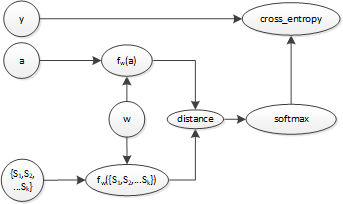
\includegraphics[scale=1]{images/Figure_5.png}
	\caption{The architecture of the mapping function $F_W$. The first three dilated-conv-dense blocks are designed to enhance the robust representation of the skeleton image. Meanwhile, the later three convolution blocks are for projecting the feature into a discriminative space. And the final flatten layer will convert the feature into a one-dimension tensor. Weights and biases of the network are corresponding to the parameter of the mapping function.}
	\label{fig:5}	
\end{figure}

\begin{algorithm}[htb]
	\caption{the training process of action recognition model.}
	\KwIn{
		$k$ classes of labeled sample $A=\{A^1,A^2,\cdots A^k\}$, where the i-th class of sample $A^i=\{a_1^i,a_2^i,\cdots a_N^i\}$ is labeled as $y^i$ and the $N_s$ and $N_q$ are the quantity of the support and query samples.
	}
	\KwOut{$W$}
	\label{alg:2}
	\bf{Init $W$}

	
	\Repeat{}
	{
			\ForEach{\bf{i in K}}
		{
			$\mathbf{I^i}=\{I^i_1,I^i_2,\cdots I^i_N\}=\mathbf{encode}(S^i)$
			
			$\mathbf{F^i}=\{F^i_1,F^i_2,\cdots F^i \{ N_s \} \}=\mathbf{F_w(I^i)}$
		}	
		\ForEach{\bf{i in K}}
		{
			$F^i_{supprot}\leftarrow RandomSample(F^i,N_s)$
			
			$F^i_{query}\leftarrow F^i\-- F^i_{support}$
			
			$c_i\leftarrow mean(F^i_{support})$
		}
		$C_{support}\leftarrow \{c_1,c_2,\cdots c_k\}$
		
		$J\leftarrow0$
		
		\ForEach{\bf{i in K}}
		{
			\ForEach{\bf{$F_{it}$ in $F^i_{query}$}}
			{
				
				$J\leftarrow J+ \frac{1}{N_q*K}log\{p(y^i|F_it,C_{support},W)\}$
			}	
		}
		$W^{new}\leftarrow W^{old}\-- \epsilon\bigtriangledown_W J$
	}
\end{algorithm}







\section{Experiments}
As mentioned before, the whole architecture of our model is provided in Figure \ref{fig:1}. we construct the mapping function as a tiny convolution network, The structure is illustrated in Figure \ref{fig:2}. It composed of three dilated-conv-dense blocks, three convolution blocks and a flatten layer. We implemented our method on Tensorflow with GTX 1080 and evaluated it on two popular benchmarks. We train our model under few-shot setup. But it still achieves a comparable accuracy to the current existing fully supervised algorithm. Besides, we also show our model can adjust the unseen classes with a few labeled samples without retraining the parameter of the mapping function. A reproducible code is available in github. \url{https://github.com/NanYoMy/human_action_recognition}

\subsection*{UTD-MHAD}
The UTD-MHAD dataset contains 27 classes of actions performed by 8 subjects (4 females and 4 males), Each subject repeated each action 4 times. For training the model, we follow the cross-subjects protocol on this dataset~\cite{chen2015utd}. And we randomly selected 8 support samples per class from the training set to estimate the prototypes of the model. Table 1 shows the recognition accuracy of different methods on UTD-MHAD dataset. Compare to other algorithm, our method only needs 16 labeled samples per class for training without any data augmentation mechanism used in ~\cite{pham2017learning,li2017skeleton_2}, but still, we obtain an improvement of $1\%$ over the state-of-the-art .

\begin{table}[htb]
	\begin{center}		
		\begin{tabular}{|c|c|}
			\hline
			Method & Accuracy \\
			\hline\hline
			ELC-KSVD & 76.19\% \\
			kinect \& Inertial & 79.10\% \\
			Cov3DJ & 85.58\%\\
			SOS & 86.97\% \\
			JTM & 87.90\% \\
			TSIIM-MSDCNN[21] & 96.27\% \\
			Our Model & \bf{97.62\%} \\
			\hline
		\end{tabular}	
	\end{center}		
	\caption{ comparison of different action recognition methods on UTD-MHAD.}
	\label{tab:1}
\end{table}

\subsection*{KARD}
The KARD~\cite{gaglio2015human} dataset contains 18 actions, performed by 10 subjects and each subject repeated each action 3 times for creating a number of 540 sequences. Following the evaluation protocol in ~\cite{pham2017learning}, the whole dataset is divided into three subsets. For each subset,  samples is used for training in our model and the rest is for testing. Our model requires less training examples than existing algorithm with a comparable accuracy. Furthermore, we also train our model on the whole KARD dataset. Although the quantity of the action is increased to 18, the model still achieves $99.38\%$ recognition accuracy.

\begin{table}[htb]
	\begin{center}
		\scalebox{1.1}
		{
			\begin{tabular}{|c|c|c|c|}
				\hline
				Method & Exp1 & Exp2 & Exp3 \\
				\hline\hline
				Gaglio et al. & 89.73\% & 94.50\%&88.27\%\\
				Cippitelli et al.; P = 11 & 96.47\% & 98.27\% & 96.87\%\\
				Ling et al. & 98.90\% & 99.60\% & 99.43\%\\
				DRNN[2] & 99.87\% & 98.27\% & 96.87\%\\
				\textbf{Our Model} & \textbf{99.37\%} & \textbf{99.72\%} & \textbf{99.37\%} \\
				\hline
				\textbf{Our Model} &  \multicolumn{3}{|c|}{\textbf{99.38\%}}\\
				\hline
			\end{tabular}
		}
	\end{center}
	\caption{ comparison of different action recognition methods on KARD. }
	\label{tab:2}
\end{table}

\subsection*{UNSeen Action Dataset}
To investigate the performance of the model when dealing with the samples from the unseen classes, we must evaluate it with the action that have not presented during the training phase. For this purpose, the all class of the dataset is split into two disjoint sets as showed in Table \ref{tab:3}. The parameters of the mapping function are optimized on training set. For evaluation, we randomly select a few(one) support samples per class from the testing set to estimate the prototype of the classes. And the rest testing samples are used to validate the accuracy. Table \ref{tab:4} gives the performance of the model on the unseen action without retraining the parameter of the mapping function. 

\begin{table}[htb]
	\begin{center}
		\begin{tabular}{|c|p{4.8cm}|p{4cm}|}
			
			\hline
			Dataset & Training Set  & Testing Set \\
			\hline\hline
			UTD-MHAD & (1) right arm swipe to the left, (2) right arm swipe to the right, (3) right hand wave, (4) two hand front clap, (5) right arm throw, (6) cross arms in the chest, (7) basketball shoot, (8) right hand draw x, (9) right hand draw circle (clockwise), (10) right hand draw circle (counter clockwise), (11) draw triangle, (12) bowling (right hand), (13) front boxing, (14) baseball swing from right, (15) tennis right hand forehand swing, (16) arm curl (two arms), (17) tennis serve & (18) two hand push, (19) right hand knock on door, (20) right hand catch an object, (21) right hand pick up and throw, (22) jogging in place, (23) walking in place, (24) sit to stand, (25) stand to sit, (26) forward lunge (left foot forward), (27) squat (two arms stretch out)\\
			\hline
			KARD & (1) Horizontal arm wave, (2) High arm wave
			(3) Two hand wave, (4) Catch Cap, (5) High throw, (6) Draw X, (7) Draw Tick, (8) Toss Paper, (9) Forward Kick, (10) Side Kick
			& (11) Take Umbrella, (12) Bend, (13) Hand Clap, (14) Walk, (15) Phone Call, (16) Drink, (17) Sit down, (18) Stand up \\
			\hline
		\end{tabular}	
	\end{center}
	\caption{ list of action in two disjoint sets (training set and testing set). }	
	\label{tab:3}
\end{table}
\begin{table*}[htbp]
	\begin{center}	
		\begin{tabular}{|c|c|c|}
			\hline
			& UTD-MHAD & KARD\\
			\hline\hline
			5 support samples & 93.5\% & 95.88\% \\
			1 support samples & 82.54\%
			& 87.3\%\\
			\hline
		\end{tabular}	
	\end{center}
	\caption{ the classification accuracies of the model with different number of support samples on UTD-MHAD and KARD datasets. All accuracy result is averaged over 1000 randomly selection of the support samples. }	
	\label{tab:4}
\end{table*}


\section{Conclusion}
We present an action recognition method based on a few shot learning. It can achieve a comparable performance even with a few training samples. And we also demonstrate that our method can classify the unseen actions without retrain the parameter of the model. But, the ability of the model is limited, our method cannot be applied to the long-term skeleton sequence, which may contain a different type of continue actions. In the future, we will extend our action recognition task to the segmentation of the long-term skeleton sequence based on the few shot learning.

%-------------------------------------------------------------------------
\section{Acknowledgment}
This work was supported in part by the Educational research projects for young and middle-aged teachers of Fujian under Grants JAT170796


%-------------------------------------------------------------------------
%



\bibliography{egbib}
\end{document}
